General relativity describes how the fabric of space and time is bent by the presence of matter and energy.
It was first written down by Einstein more than a hundred years ago, and is to this day the most accurate model we have for gravitational effects.
The theory has made numerous accurate and counterintuitive predictions, which have been borne out by experiments.
In this chapter, we will survey the basics of general relativity as well as some mathematical prerequisites.
We will then use this to derive the Tolman-Oppenheimer-Volkoff (TOV) equation.
This is a differential equation that models massive stellar objects, such as stars. 
This chapter is based on~\autocite{carrollSpacetimeGeometryIntroduction2019,leeSmoothManifolds2012}.

\section{Differential geometry}

General relativity is formulated in the language of \emph{differential geometry}, which generalizes multivariable calculus to more general spaces than $\R^n$.
Such a space is a differentiable \emph{manifold}, $\Em$.
A manifold is a set of points that are locally homeomoriphic to $\R^n$.
That is, for all points $p \in \Em$, there is a neighbourhood $U$ around $p$ and a corresponding set of continous functions,
\begin{align}
    x^\mu: U \subseteq \Em & \longmapsto V \subseteq \R^n, \\
    p & \longmapsto x^\mu(p).
\end{align}
that has a continous inverse-functions $\varphi_x$ such that $\varphi_x(x(p)) = p$ for all $p \in U$.
$x^\mu = (x^0, ..., x^{n- 1})$ are a coordinate function of $\Em$.
In the case of a differentiable manifold, these must be diffeomorphisms, i.e. infinitly differentiable.
Differentiablility of coordinate functions is defined by considering two different coordinate functions, $x^\mu$ and $x'^\mu$, with the possibliy overlapping domains $U$ and $U'$.
We can then define a function between subsets of $\R^n$ by mapping via $\Em$, the transition map  
\begin{align}
    f_{x'\rightarrow x} = x^\mu\circ\varphi_{x'} : \R^n \mapsto \R^n.
\end{align}
%
It is defined as the function which makes the following diagram commute\footnote{To be rigorous, one has to restrict the domains and image of the coordinate function when combining them. We will leave this implicit here.}
%
\begin{equation}
    \begin{tikzcd}
        \R^n \arrow[rd, "f_{x'\rightarrow x}"'] & \Em \arrow[l, "x"'] \arrow[d, "x'"] \\
        & \R^n
        \end{tikzcd}
\end{equation}
%
The map is illustrated in \autoref{fig: transition map}.
A set of functions $\mathcal A = \{x^\mu\}$ whose domain cover $\Em$ is called an \emph{atlas} of $\Em$.
If the transition function between \emph{any} two coordinate functions in the atlas is smooth, then we call the atlas smooth.
To uniquily define a differentiable manifold,  form smooth transition functions form an \emph{atlas} $\mathcal{A}$.
We then define a differentiable, or smooth, manifold as the topological manifold $\Em$ together with the \emph{maximal} atlas $\mathcal A$.
A smooth atlas is maximal if no other coordinate function can be added to the atlas while it retains its smoothness.\footnote{The maximal condition is to ensure that two equivalent atlases correspond to the same differentiable manifold. A single manifold can be combined with different maximal atlases, also called differentiable structures. }
%
\begin{figure}
    \centering
    \includegraphics[width=0.5\textwidth]{figurer/transition_map_kladsvg.pdf}
    \caption{Kladd: The transition map between two coordinates}
    \label{fig: transition map}
\end{figure}

Consider two $m$ and $n$ dimensional smooth manifolds $\Em$ and $\mathcal N$.
Let $x$ denote the coordinates on $\Em$, while $y$ denotes the coordinates on $\mathcal N$.
We can define smooth functions between these manifolds in a similar way.
Consider the function
%
\begin{equation}
    F: \Em \longmapsto \mathcal N.
\end{equation}
%
This is said to be smooth, if for all points $p \in M$, there is a set of local coordinates $x$ around $p$ and $y$ around $F(p)$ so that the map $\tilde F = y \circ F \circ x^{-1}$ is smooth.
This map is defined by the diagram
%
\begin{equation}
    % https://tikzcd.yichuanshen.de/#N4Igdg9gJgpgziAXAbVABwnAlgFyxMJZABgBoBGAXVJADcBDAGwFcYkQAdDgW3pwAsARoIAEAJQB63EAF9S6TLnyEUZYtTpNW7LrwEBjJiICys+SAzY8BIuVLqaDFm0SceffocYiAcmYVWyrYUGk7arroewuIShDIaMFAA5vBEoABmAE4Q0oh2IDgQSGQgjPSCMIwACorWKqUw6TggjlouIAAe-iBZOUj5hUgATK3O7OndvbkjBUWIAMyj4SAAnpPZuSWDC0vtSbKUMkA
\begin{tikzcd}
    \mathcal M \arrow[d, "x"] \arrow[r, "F"] & \mathcal N \arrow[d, "y"] \\
    \mathbb R^m \arrow[r, "\tilde F"]               & \mathbb R^n              
    \end{tikzcd}
    %
\end{equation}
%
%
We will not be careful with  the distinction between $F$, the funciton between the abstract manifolds, and $\tilde F$, the function of theri coordinates, but rather denote both by $F(x)$.
We may take the partial derivative of such a function with respect to the coordinates $x$, $\diffp{F}/{x^\mu}$.
However, this is obviously dependent on our choice of coordinates, as a set of local coordinates can always be scaled.
To get a coordinate-independent quantity, we have to introduce the tangent space and the metric.

\subsection*{Vectors and tensors}

A curve $\gamma$ through $\Em$ i a function from $\R$ to $\Em$,
%
\begin{align}
    \gamma : \R &\longmapsto \Em \\
    \lambda & \longmapsto \gamma(\lambda).
\end{align}
%
Such curves are often denote only by their coordinates and the parameter $\lambda$, $x^\mu(\lambda) = (x^\mu \circ \gamma)(\lambda)$.
Such a curve defines a directional derivative of a real valued function $f: \Em \mapsto \R$.
Assume $\gamma(\lambda = 0) = p$.
As we are always taking the derivative of functions between $\R^n$, for different $n$, we can use the chaine rule.
The directional derivative of $f$ at $p$, given by this curve $\gamma$, is then
%
\begin{equation}
    \diff{}{\lambda} f(x(\lambda)) \bigg |_p = \diff{x^\mu}{\lambda} \bigg |_{\lambda = 0}  \diffp{}{x^\mu} f(x) \bigg |_p.
\end{equation}
%
The set of all such directional derivatives at $p$ form a vector space, $T_p \Em$, called the \emph{tangent space}.
The coordinates $x^\mu$ induce a basis of this vectorspace, 
%
\begin{equation}
    e_\mu = \diffp{}{x^\mu} = \partial_\mu,
\end{equation}
%
so any element $v \in T_p \Em$ can be written
%
\begin{equation}
    v = v^\mu \partial_\mu = \diff{x^\mu}{\lambda} \diffp{}{x^\mu}.
\end{equation}
%
Her, $\lambda$ is the parameter of the curve corresponding to the directional derivative $v$.\footnote{There is not only one curve corresponding to any directional derivative, but rather an equivalence class. }
It acts on funcitons $f : \Em \mapsto \R$ as
%
\begin{equation}
    v(f) = v^\mu \partial_\mu f.
\end{equation}
%

A function $F$ between two manifolds $\Em$ and $\mathcal N$ also induces a map between the tangent spaces of these manifolds.
This is the \emph{differential} of $F$ at $p$, 
%
\begin{align}
    \dd F_p: T_p \Em & \longmapsto T_p \mathcal N.
\end{align}
%
This is a directional derivative on $\mathcal N$, and is defined as
%
\begin{equation}
    \dd F_p(v) (g) = v(g \circ F),
\end{equation}
%
for functions $g : \mathcal N \mapsto \R$.
It thus acts on funcitons on $\mathcal N$ by ``extending'' the derivative $v$.
This is a linear map between vectorspaces, an may be written on component form by considering the differentials of the coordinate functions.
Denote the coordinates of $\mathcal N$ by $y^\mu$, and $y^\mu \circ F = F^\mu$.
Then,
%
\begin{equation}
    \dd F_p (\partial_\mu) (g) = \partial_\mu (g \circ F) |_p 
    = \diffp{F^\nu}{x^\mu}\bigg |_p \diffp{g}{y^\nu} \bigg  |_{F(p)}
\end{equation}
%
The differential is thus a generalization of the Jacobian of a function.
In the cas where of a real valued funciton, $f: \Em \mapsto \R$, and $g : \R \mapsto \R$, we get
%
\begin{equation}
    \dd f_p (v) (g) 
    = v(g \circ f) 
    = (v^\mu \partial_\mu f) |_p \, \diff{g}{f}\bigg  |_{f(p)},
\end{equation}
%
or more simply
%
\begin{equation}
    \dd f_p (v) = v^\mu \partial_\mu f |_p
\end{equation}
%
The differential of a real-valued function is thus a linear map from the vector-space $T_p \Em$ to the real numbers.
The set of all such maps form the \emph{dual space} of $T_p \Em$, denoted $(T_p^* \Em)$.
We can regard each of the coordinate functions as a real valued function,
%
\begin{equation}
    \dd x^\mu (\partial_\nu) = \diffp{x^\mu}{x_\nu} = \delta^\mu_\nu.
\end{equation}
%
These form a basis for $T^*_p \Em$.
We can show this by assuming $v = v^\mu \partial_\mu \in T_p \Em$.
Then, assuming $\dd f_p = \omega_\mu \dd x^\mu$, we get
%
\begin{equation}
    \dd f (v) = v^\mu \partial_\mu f = v^\mu \omega_\nu \dd x^\nu(\partial_\mu) = v^\mu \omega_\mu.
\end{equation}
%
Thus, we obtain a rigorous just justification for the classical expression 
%
\begin{equation}
    \dd f = \diffp{f}{x^\mu} \dd x^\mu,
\end{equation}
however we now interpret it as a covector-field instead of an ``infinitesimal displacement''.

This linear map from vectors to real numbers is gerneralized by \emph{tensors}.
Given a vector space $V$, general $(n, m)$ tensor $T$ is a multilinear map, which associates $n$ elements from $V$ and $m$ from its dual $V^*$ to the real numbers, i.e.
%
\begin{align}
    T: V \times V \times .... \times V^* \times .... &\longmapsto \R, \\
    (v, u...; \omega, ...) & \longmapsto T(v, u, ...; \omega, ...).
\end{align}
%
Multilinear means that $T$ is linear in each argument.
The set of all such maps is the tnesor product space $V\otimes V \otimes ... \otimes V^* \otimes ...$, a $\dim(V)^{n+m}$-dimensional vector space.
If $\{e_\mu\}$ and $\{e^\mu\}$ are the basis for $V$ and $V^*$, then we can write the basis of this of the tensor product space as $ \{e_\mu \otimes... e^\mu \otimes ... \}$.
The tensor can thus be written
%
\begin{equation}
    T = T^{\mu \nu\dots}{}_{\rho\dots} \, e_{\mu}\otimes e_\nu \otimes \dots e^\rho\otimes\dots, 
\end{equation}
%
where
%
\begin{equation}
    T^{\mu \nu\dots}{}_{\rho\dots} = T(e^\mu e^\nu, \dots; e_\rho, \dots).
\end{equation}


\subsection*{Geometries and the metric}

The metric is a symmetric, non-degenerate $(0, 2)$ tensor
%
\begin{equation}
    \dd s^2 = g_{\mu \nu} \, \dd x^\mu \otimes \dd x^\nu.
\end{equation}
%
It defines the geometry of the manifold $\Em$, and is the main object of study in general relativity.
As it is invertible, we define $g^{\mu \nu} = (g^{-1})_{\mu \nu}$, which is the components of a $(2, 0)$ tensor.
We use this to raise and lower indecies, as is done with the Minkowski metric $\eta_{\mu \nu}$ in special relativity.

Up until now, we have studied the tangent space $T_p \Em$ at one point, and the correpsonding dual and tensor product spaces.
We are, however, more interested in feilds of vectors, covectors and tensors than.
A tensor field $T$ takes the a value $T(p)$ of the tensor product space corresponding to the tangentspace at $p\in \Em$, $T_p \Em$.
We will use a vector felt to illustrate.
This vector field can be written as
%
\begin{equation}
    v(p) = v^\mu(p) \partial_\mu |_p. 
\end{equation}
%
We will mostly be working with the compontets $v^\mu$, which are functions of $\Em$.
For ease of notation, we write the vector as a funciton of the coordinates $x$, and drop leave the evaluatation at $p$ implicit.
The vector field $v(x)$ is unchanged by a coordinate-transformation $x^\mu \rightarrow \tilde x^\mu$; the coordinate has no effect on it and is only for our convinience. 
With this, we can deduce the transformation rules of the components under such a transformation:
%
\begin{equation}
    v = v^\mu \partial_\mu = v^\mu \diffp{\tilde x^\nu}{x^\mu} \tilde  \partial_\nu
    = \tilde v^\mu \tilde \partial_\mu, 
\end{equation}
%
or
%
\begin{equation}
    \tilde v^\mu = \diffp{\tilde x^\mu}{x^\nu} v^\nu.
\end{equation}
%
For covectors, it is
%
\begin{equation}
    \tilde \omega_\mu = \diffp{x^\nu}{\tilde x^\mu} \omega_\nu
\end{equation}
%
The gradient of a scalar function $f$, $\dd f = \partial_\mu f \dd x^\mu$, is a coordinate-independent derivative, as $\partial_\mu f$ follows the transformation law for covectors.
We generalize this by introducing the covariant derivative, $\nabla$, as a map from $(n, m)$ tensor fields to $(n, m+1)$ tensor fields.
When considering a scalar as a $(0, 0)$ tensor, we see that this generalizes the scalar derivative.

We assume
%
\begin{itemize}
    \item linearity: $\nabla (T + S) = \nabla T + \nabla S$.
    \item product rule: $\nabla (T \otimes S) = (\nabla T)\otimes S + T \otimes (\nabla S)$.
    \item reduces to partial derivative: $\nabla_\mu f = \partial_\mu f$.
    \item Krönecker delta gives zero: $\nabla_\mu \delta^\rho_\nu = 0$.
\end{itemize}
%
With this, we can in general write the covariant derivative as~\autocite{carrollSpacetimeGeometryIntroduction2019}
%
\begin{align}
    \nabla_\mu v^\nu &= \partial_\mu v^\mu + \Gamma^\mu_{\nu \rho} v^\rho, \\
    \nabla_\mu \omega_\nu &= \partial_\mu \omega_\nu - \Gamma^\rho_{\mu \nu} \omega^\rho,
\end{align}
%
for vectors and covectors.
$\Gamma^{\mu}_{\nu \rho}$ are called \emph{Christoffel symbols}.
The generalization for higher-order tensors is straight forward, 
%
\begin{equation}
    \nabla_\mu T^{\nu\dots}{}_{\rho\dots}
    =
    \partial_\mu T^{\nu\dots}{}_{\rho\dots}
    + \Gamma^\mu_{\nu \lambda} T^{\lambda\dots}{}_{\rho\dots} +\dots
    - \Gamma^\lambda_{\mu \rho} T^{\mu\dots}{}_{\lambda\dots} -\dots
\end{equation}
%
This is still not enough to to uniquely determin the Christoffel symbols.
We will furhtermore assume $\Gamma^{\lambda}_{\mu \nu} = \Gamma^{\lambda}_{\nu \mu}$ and $\nabla_\mu g_{\nu \rho} = 0$.
With these, we can find an explicit formula of the Christoffel symbols in terms of the metric, 
%
\begin{equation}
    \label{christoffel symbols from metric}
    \Gamma^\rho_{\mu \nu} = \frac{1}{2} g^{\rho \sigma} (\partial_\mu g_{\nu \sigma} - \partial_\sigma g_{\mu \nu} + \partial_{\nu}g_{\sigma \mu}).
\end{equation}
%

The curvature of the manifold $\Em$, with the metic $g_{\mu \nu}$, is encoded in the Riemann tensor.
It is defined by
%
\begin{equation}
    [\nabla_\mu, \nabla_\nu] v^\rho = R^{\rho}{}_{\sigma \mu \nu} v^\sigma,
\end{equation}
%
which in our case gives the explicit formula
%
\begin{equation}
    \label{riemann tensor in terms of christoffel symbols}
    R^\rho{}_{\sigma \mu \nu} 
    = \partial_{\mu} \Gamma^{\rho}_{\nu \sigma}
    - \partial_{\nu} \Gamma^{\rho}_{\mu \sigma}
    + \Gamma^{\rho}_{\mu \lambda} \Gamma^{\lambda}_{\nu \sigma}  
    - \Gamma^{\rho}_{\nu \lambda} \Gamma^{\lambda}_{\mu \sigma} 
\end{equation}
%
Although the Christoffel symbols are not tensors, this quantity is a well-defined tensor due to its definition using covariant derivatives.
We can therefore contract some of its indices to get other tensor quantities.
We  define the Ricci tensor and Ricci scalar as
%
\begin{align}
    \label{Ricci tensor}
    R_{\mu \nu} &= R^{\rho}{}_{\mu \rho \nu}, \\
    \label{Ricci scalar}
    R &= R^{\mu}{}_{\mu} = g^{\mu \nu} R_{\mu \nu}.
\end{align}
%
These are the quantities we need to start working with general relativity.

\subsection*{Integration on manifolds}

The integral of an scalar function on a manifold is not a coordinate independent notion, and we must instead introduce the notion of $n$-forms.
A $n$-form is a antisymmetric $(0, n)$ tensor.
To ease notation, we introduce the symmetrization of
%
\begin{equation}
    T_{(\mu_1\dots\mu_n)} 
    = \frac{1}{n!} \sum_{\sigma \in S_n} 
    T_{\mu_{\sigma(1)} \dots \mu_{\sigma(n)}},
\end{equation}
%
where $S_n$ is the set of all permutations of $n$ objects.
The antisymmetrization of a tensor is defined as
%
\begin{equation}
    T_{[\mu_1\dots\mu_n]} 
    = \frac{1}{n!} \sum_{\sigma \in S_n} \text{sgn}(\sigma)  
    T_{\mu_{\sigma(1)]} \dots\mu_{\sigma(n)}}.
\end{equation}
%
The components of a $n$ form then obey $T_{\mu_1 \dots \mu_n} = T_{(\mu_1 \dots \mu_n)}$.
We are interested in the volume one-form, or measure, and therefore define
%
\begin{equation}
    \dd^n x = \dd x^0 \wedge \dots \wedge \dd x^{n-1}.
\end{equation}
%
Here, $\wedge$ is the wedge product, defined as
%
\begin{equation}
    (A\wedge B)_{\mu_1\dots\mu_{n+m}} = \frac{(n + m)!}{n! m!} A_{[\mu_1\dots\mu_n}B_{\mu_{n+1}\dots\mu_{n+m}]},
\end{equation}
%
and $\dd x^i$ is the one-form corresponding to the $x^0$-coordinate function.
Given a different set of coordinates, $\tilde x^\mu$, these are related by
%
\begin{equation}
    \dd^n x = \det\left(\diffp{x}{\tilde x} \right) \dd^n \tilde x,
\end{equation}
%
by the properties of the wedge product.
This quantity is a tensor-density, rather than a tensor, as it scales as $|\det(\diffp{x}/{\tilde x})|$.
To make the measure coordinate independent, we must multiply with a scalar density to conpensate.
By the transformation properties of tensors, $\sqrt{|g|} = \sqrt{| \det(g_{\mu\nu})|}$  will do just this.
We therefore define the integral of a scalar function $f$ on a manifold $\Em$ as
%
\begin{equation}
    I = \int_{\Em} \dd^n x \, \sqrt{|g|} f(x).  
\end{equation}


Stoke's thorem generalizes the fundamental theorem of calculus, as well as the divergence theorem, to manifolds.
Let $\Em$ be a differential manifold of dimension $n$, with the boundary $\partial \Em$.
The boundary is then $n-1$ dimensional, and a metric $g$ on $\Em$ will induce a new metric $\gamma$ on $\partial \Em$, and there will be a vector field $n^\mu$ of normalized vectors orthogonal to all elements of $T \partial \Em$.
The generalized divergence theorem then states that, for a vector field $V^\mu$ on $\Em$,
%
\begin{equation}
    \int_\Em \dd^n x \, \sqrt{|g|} \,  \nabla_\mu V^\mu 
    = \int_{\partial \Em} \dd^{n-1}y \, \sqrt{|\gamma|} \, n_\mu V^\mu.
\end{equation}
